\documentclass[11pt]{article}
\usepackage{booktabs}
\usepackage{graphicx}
\title{CSC 464 Project}
\author{Sterling Laird - V00834995}
\date{December 14th 2018}

\graphicspath{ {../diagrams/} }

\begin{document}

\maketitle

\section{Introduction}
For my project, Ic hose  to implement the Logoot CRDT and a simple peer-to-peer document editing client using the CRDT. This report covers the basics of my implementation as well as my evaluation of the work done so far.\\

All code in this project was written by me, Sterling Laird with most of my knowledge of the algorithms implemented coming directly from \textit{Logoot: A Scalable Optimistic Replication Algorithm for Collaborative Editing on P2P Networks} (Weiss, Urso, \& Molli, 2009) and from various online sources outlining the algorithms used to solve these problems such as \textit{stackoverflow.com}. All implementations can be found on my Github page \\(https://github.com/sterlinglaird/CSC-464).

\pagebreak

\section{Implementation}
To implement my project, I chose  the language Go because of the simple concurrency constructs, as well as so I can learn more about the language.

\subsection{Logoot CRDT}
In Logoot, elements in a document have a total ordering property which helps ensure that peers can modify the document with arbitrary latency and all peers will reach eventual consistency of their own local copies. Each element in a Logoot CRDT has a positional index that is fixed regardless of surrounding insertions and deletions. When an insertion of an element $I$ is done between any two elements $A,B$ the resulting position of $I$ is $pos(A) < pos(I) < pos(B)$. Similarly when deleting elements, the surrounding elements are undisturbed. The positional indexes are implemented with a list of positions representing digits in a arbitrary base so that all positions can be considered a real number that exists between between $0$ and $maxdigit$. I chose to use base $2^8=256$ as larger numbers can make testing difficult as with a larger base, you need exponentially more elements to create a the same maximum length of the digits list. Using a higher base decreases the length of each positions digits on average, but increases the minimum memory of each element.\\


To implement the CRDT, I created a small Go package \textit{document} containing all of the code needed to represent a document using the Logoot algorithm. To use the CRDT, a user simply needs to create a new document and a new position at the start of the document. When the user wants to insert an element between two existing elements, they simply use the Move() function to move the current position to where they want to insert the new element, and then use the  InsertRight() or InsertLeft() functions to insert the new element to the right or left respectively of the current position. These functions will then return the newly created position and the process can repeat. When an element needs to be deleted a similar process occurs, the user moves the position to the element next to the soon to be deleted element, and calls the DeleteRight() or DeleteLeft() functions to delete the element on either side. Additionally there is a logical clock which is incremented on each operation and every insert is marked with the logical logical clock to resolve conflicts when the positions of two elements are the same.

\begin{center}
	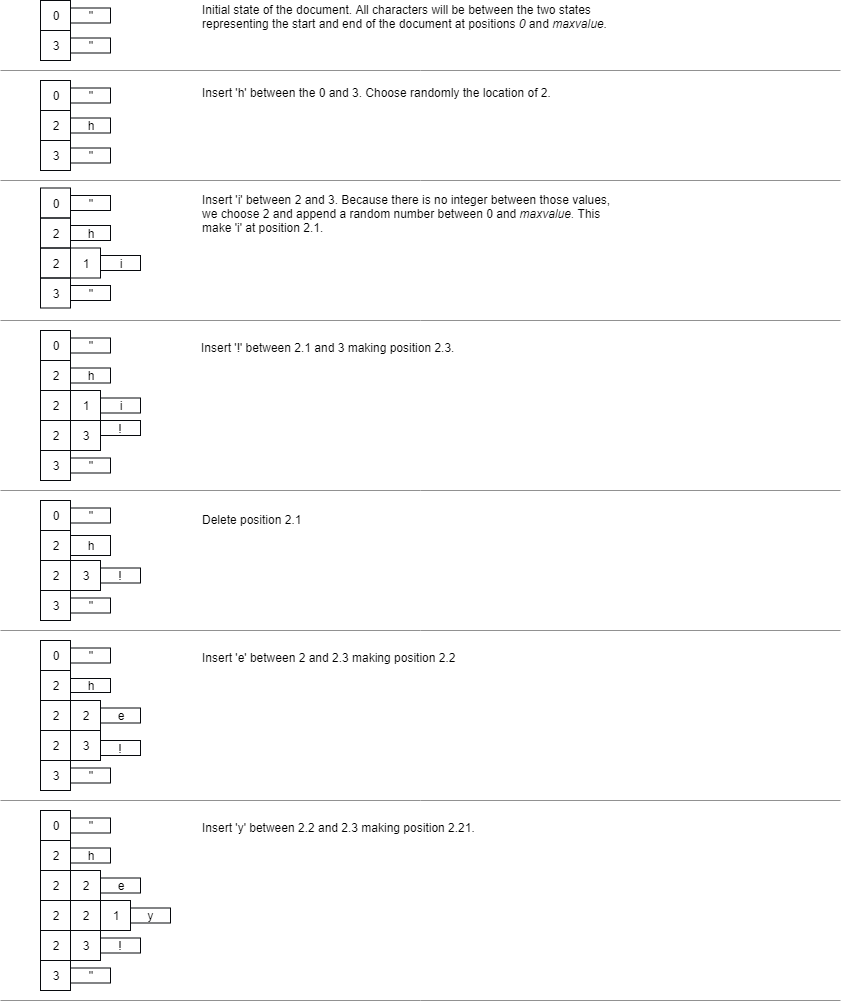
\includegraphics[scale=0.5]{document.png}\\
	A basic example of inserting and deleting elements into a Logoot document with base 4.
\end{center}



\subsection{Client}
To provide a practical application of the Logoot CRDT, I implemented a simple peer-to-peer document edition client to help show the usefulness of the CRDT. The client (\textit{app.go}) is a simple console-based text editor that uses the \textit{TermBox-Go} library for the user interface.\\

When starting the program the user passes in command line arguments specifying the port they will like to listen on, and optionally the addresses/ports of the other clients they want to collaborate with. When clients are connected, all modifications they make to their local copy of the document will the transmitted to all the other peers whose local documents will update in a consistent fashion. Currently, the only actions supported by the client GUI are insert character, delete character, insert new line, move cursor, and close editor using CTRL-C. This is a very basic set of actions but is sufficient to show the usefulness of the CRDT.

\begin{center}
	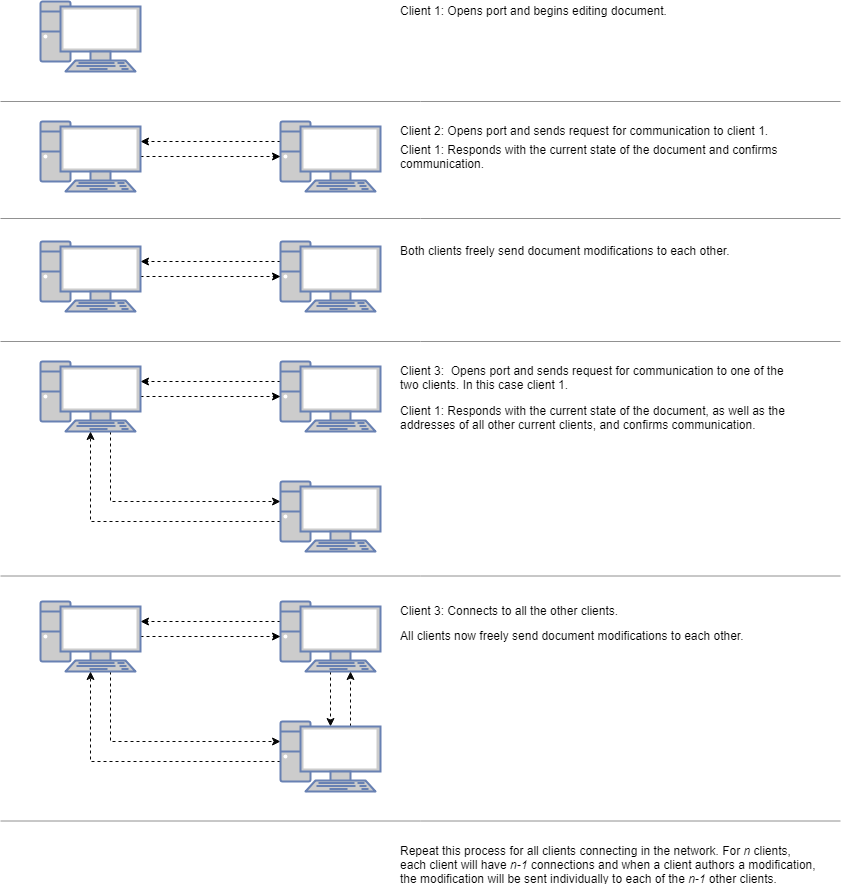
\includegraphics[scale=0.5]{connecting.png}\\
	The process of clients joining the network to collaborate on a shared document.
\end{center}

\begin{center}
	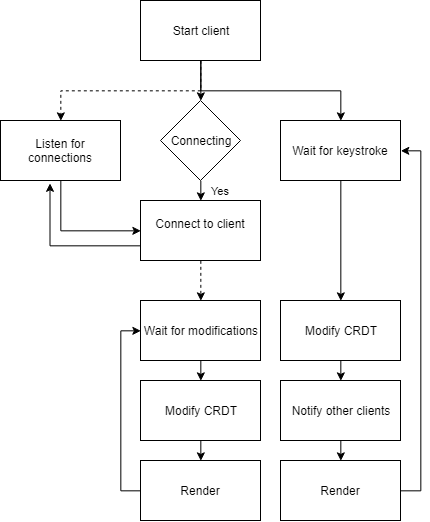
\includegraphics[scale=0.75]{client.png}\\
	The general flow chart of the client. Dotted lines represent new threads of execution
\end{center}

\pagebreak

\section{Evaluation}
In order to test the functionality of the CRDT in the most basic case, where there is only a single user, I created two fuzz/unit testing functions, one of which tests the ability to insert new elements, and the other tests the ability to insert and delete elements. Both of these functions are currently set up to each run 1000 random operations and each are run 1000 times with a different random seed each time. As no failures are arising, I am cautiously optimistic that my implementation is correct thus far. Due to time constraints, parts of my code are not ideal in terms of code quality, so it is currently difficult to logically verify my results. Both of the tests I run are considered a success by maintaining a separate copy of what we would expect the document to look like after each operation, if a discrepancy between the Logoot document and the separate copy are found, an error will be reported. Keeping a separate copy is a feasible strategy for testing these features because we are not testing any concurrency related features in a simulated peer to peer network. Because of this we can fairly trivially implement a data structure which the keeps relative ordering consistent (for testing) with insertion and deletion operations, but fails to keep absolute positions as Logoot does.\\

In order to test the CRDT with concurrent operations that may have latency, I started to create a similar testing suite as the one above for sequential operations. These testing functions perform operations concurrently before sending the operations to other replicas with random latency. The tests make sure that after all the operations have been successfully transmitted to all other replicas, all replicas have the same document. Unfortunately due to time constraints I couldn't fully finish this testing suite so in lieu of automated testing I manually tested the client code with random latency ($>$1 second) and with 4 clients in a network and could not find failures in consistency from those tests. Of course this does not mean there are not cases where they would fail, but it does give some level of assurance.


\pagebreak

\section{Further Work}
There is much more further work to be done to improve my implementation. As mentioned previously, I have yet to complete an automated concurrency based test for consistency between replicated copies of the document. Completing that test would provide an additional level of assurance that the program works as intended. Additionally the client program does not fully meet design goals as when a new peer connects with an already connected peer, the new client currently does not get updated with the current state of the document as well as with the addresses of the other clients. Because of this the program only works properly when a new peer lists all the other peers they want to connect with, and the document is empty until all peers are connected. Finally, my current implementation uses a base of 256 for the positional digit, this value is likely not ideal and it would be useful to test out different values and see what value reduces the amount of overhead and computation time. In the Logoot paper, the authors suggest 8-byte digits and 4-byte logical clocks.
\end{document}
